\newpage
\chapter{Фрактальные $k$-кубы, являющиеся дендритами}

В этой главе мы рассмотрим фрактальные $k$-кубы и опишем последовательность действий, по которым можно определить, является ли данный фрактальный куб дендритом с одноточечным пересечением.


\section{Пересечения копий фрактального $k$-куба}


\subsection{Фрактальные $k$-кубы}

\begin{definition}[Olsen L. (1998) \cite{Olsen1998}; Lau K., Luo J.J.,Rao H. (2013) \cite{LLR2013}]
\label{dfn:FQ}
Пусть  $D=\{d_1,\ldots,d_r\},\; d_i\in\{0,1,\ldots,n-1\}^k$, где $n\ge 2$, а $1<\#D<n^k$.\\
{\em Фрактальным $k$-кубом порядка $n$ с множеством единиц $D$} называют компактное множество $K\IN\rr^k$, удовлетворяющее равенству
\begin{equation}\label{fqeq}
K=\dfrac{K+D}{n}.
\end{equation}
\end{definition}

\begin{figure}[h!]
    \centering
    \qquad
    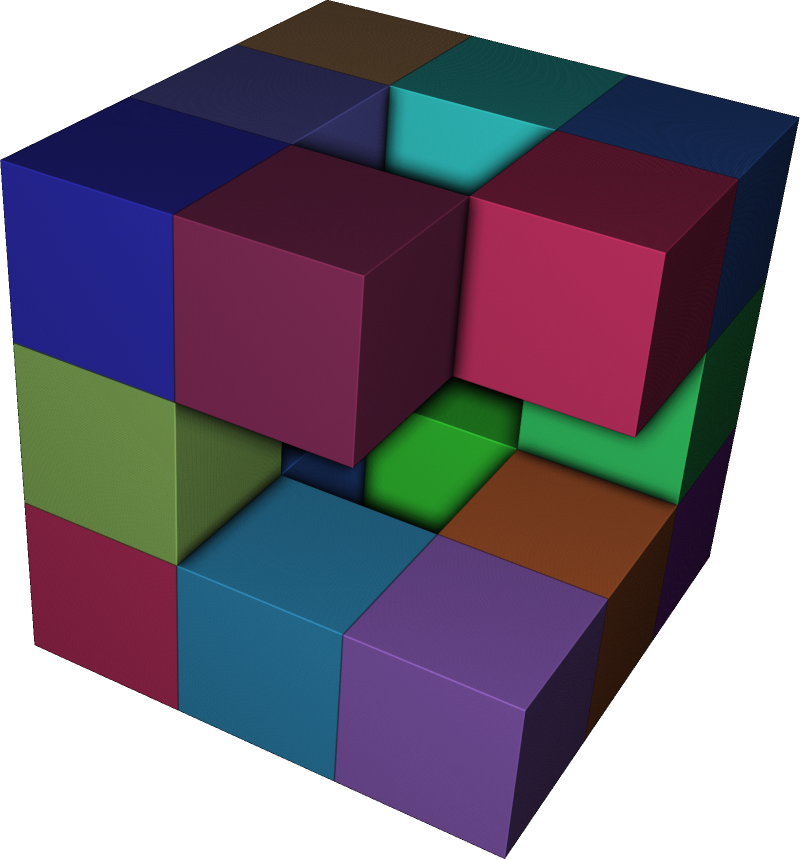
\includegraphics[width=0.4\textwidth]{FQD.png}
    \hfill
    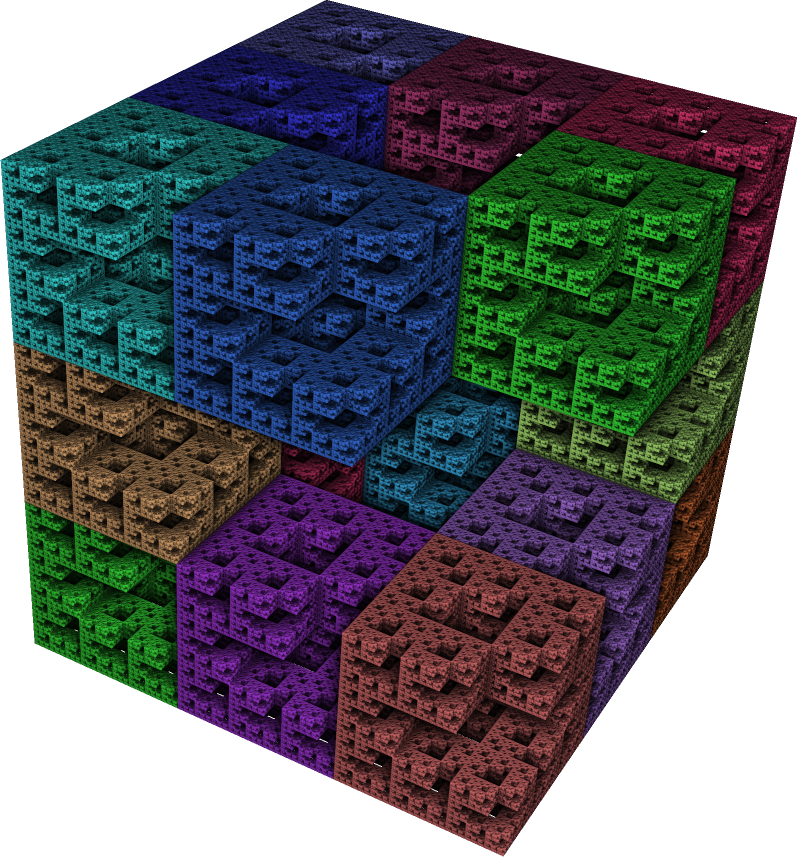
\includegraphics[width=0.4\textwidth]{FQK.png}
    \qquad
    \caption{Множество $D+P$ (слева) и фрактальный куб $nK=K+D$ (справа)}
    \label{fig:FQ}
\end{figure}

В случаях, когда $k=2$ и $k=3$, мы называем $K$ \emph{фрактальным квадратом} и \emph{фрактальным кубом} сответственно.

Уравнение \eqref{fqeq} можно использовать в его эквивалентной форме $nK=K+D$.
Само же множество $K$ содержится в единичном $k$-мерном кубе $P=[0,1]^k$, поскольку $P$ удовлетворяет уравнению $nP\NI P+D$.

Рассмотрим также эквивалентное определение фрактального $k$-куба $K$ порядка $n$ с множеством единиц $D$.
Возьмем единичный $k$-куб $P$ и разобьем его на $n^k$ равных $k$-кубов с ребром $1/n$.
Ближайшая к нулю вершина каждого маленького $k$-куба $P_i$ имеет координату вида $\dfrac{d_i}{n}$, где $d_i\in\{0,1,\ldots,n-1\}^k$.
Из этого разбиения выберем те $k$-кубы $P_i$, для которых $d_i\in D$ (см. пример на рисунке \ref{fig:FQ}).
Гомотетия, переводящая $P$ в $P_i$, имеет вид $S_i(x)=\dfrac{x+d_i}{n}$.
Тогда $K=\bigcup\limits_{d_i\in D}\dfrac{d_i+K}{n}$.

Уравнение \eqref{fqeq} задаёт систему $\eS$ гомотетий $S_i(x)=\dfrac{x+d_i}{n}$, где $d_i\in D$, а оператор Хатчинсона $T_\eS$ системы $\eS$ определяется уравнением $$T_\eS(A)=\dfrac{D+A}{n}=\bigcup\limits_{d_i\in D}\dfrac{d_i+A}{n}.$$

\begin{definition}\label{refin}
Для любого $m\in \nn$, {\em $m$-е измельчение} системы $\eS$ --- это система $\eS^m=\{S_\bi, \bi=i_1i_2\ldots i_m\in I^m\}$, где $S_\bi(x)=\dfrac{x+d_\bi}{n^m}$ и $d_\bi=n^{m-1}d_{i_1}+n^{m-2}d_{i_2}+\ldots+d_{i_m}$. 
\end{definition}

Аттрактор $K$ можно рассматривать как соответствующий системе $\eS^m$ фрактальный $k$-куб порядка $n^m$ с множеством единиц $D^m=n^{m-1}D+n^{m-2}D+\ldots+D$ и копиями $\dfrac{K+d_\bi}{n^m}$.
Оператор Хатчинсона $T_\eS^m$ этой системы $\eS^m$ определяется уравнением $T_\eS^m(A)=\dfrac{D^m+A}{n^m}$.

Каждой бесконечной строке $\bi=i_1i_2\ldots\in I^\8$ соответствует единственная точка $x=\pi(\bi)$, где $\pi(\bi)=\sum\limits_{m=1}^\8 \dfrac{d_{i_m}}{n^m}$.

\begin{remark}% \label{rmk:fsd}
Далее, если не указано иное, говоря {\em <<фрактальный $k$-куб $K$>>}, мы будем иметь в виду {\em <<фрактальный $k$-куб $K$ порядка $n$ с множеством единиц $D$>>}. 
\end{remark}


\subsection{Грани $K_\al$ фрактального $k$-куба}

Единичный $k$-куб $P$ является фрактальным $k$-кубом порядка $n$ с множеством единиц $D=\{0,1,\ldots,n-1\}^k$, поскольку $P=\dfrac{P+\{0,1,\ldots,n-1\}^k}{n}.$
Значит, любой фрактальный $k$-куб $K$ содержится в единичном $k$-кубе $P$.

Если фрактальный $k$-куб $K$ является аттрактором системы $\eS$, то из включения $K\IN P$ следует $S_i(K)\IN S_i(P)$ для любого $S_i\in\eS$.
Более того, для любых $S_i, S_j\in\eS$ малые $k$-кубы $S_i(P)$ и $S_j(P)$ могут пересекаться друг с другом только по своим граням.
Прообразы этих граней в $S_i(P)$ и $S_j(P)$ относительно соответственных отображений $S_i$ и $S_j$ являются парой противоположных граней в $P$.
Введём обозначения для граней $k$-куба $P$ и пересечений этих граней с фрактальным $k$-кубом $K$.

Рассмотрим множество векторов $A=\{-1,0,1\}^k$.

Заметим, что каждый из соседей $k$-куба $P$ в целочисленной решетке $P+\zz^k$ имеет вид $P+\bma$, где $\bma\in A$. При этом пересечение $P_\bma=P\cap(P+\bma)$ является единственной гранью куба $P$, относительно центра которой кубы $P$ и $P+\bma$ симметричны. 

Тем самым мы задаем  естественное  взаимно-однозначное соответствие
между множеством $A$ и множеством граней единичного $k$-куба $P=[0,1]^k$, сопоставляющее каждому $\bma\in A$ грань 
$P_\bma=P\cap(P+\bma)$ $k$-куба $P$.

\begin{figure}[h!]
 \centering
 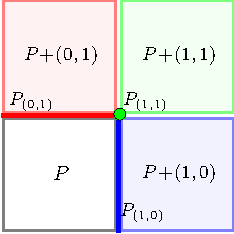
\includegraphics[width=0.45\textwidth]{faces_p.pdf}
 \hfill
 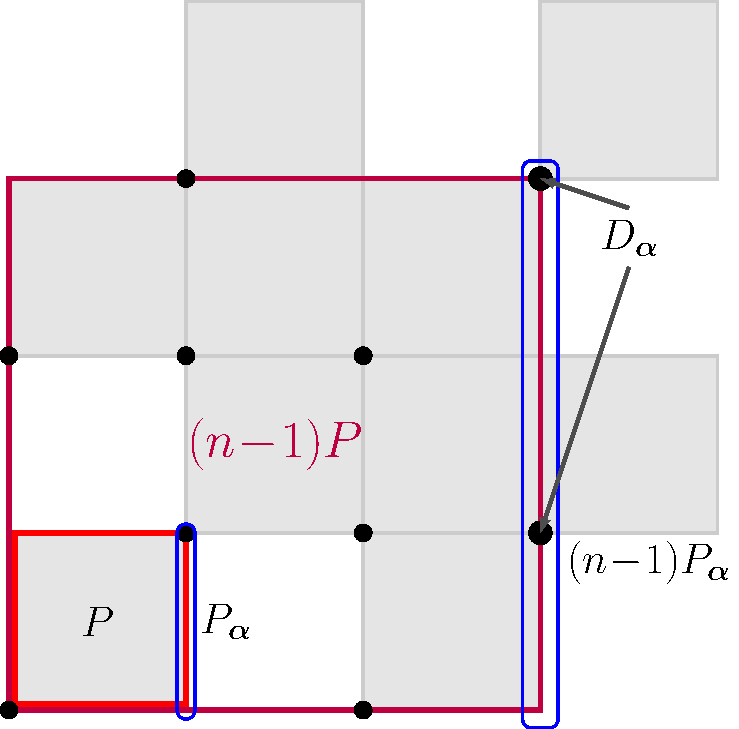
\includegraphics[width=0.45\textwidth]{faces_k.pdf}
 \caption{Множества $P_\bma$ (слева) и $D_\bma.$}
 \label{fig:faces}
\end{figure}


Симметрия противоположных граней $k$-куба $P$ выражается равенством 
$$P_\bma=P\cap(P+\bma)=((P-\bma)\cap P)+\bma=P_{-\bma}+\bma.$$

Для $\bma=(\al_1,\ldots,\al_k)\in A$  обозначим через $|\bma|=|\al_1|+\ldots+|\al_k|$ число ненулевых компонент вектора $\bma$.
Тогда вектору $\bma\in A$, при $|\bma|=l$, соответствует $(k-l)$-мерная грань $P_\bma$ $k$-куба $P$, где $k-l$ есть число равных нулю элементов вектора $\bma$.

\begin{remark}\label{rmk:point}
Для $\bma=(\al_1,\ldots,\al_k)\in A$ грань $P_\bma$ можно представить как множество точек 
$$P_\bma=\left\{x=(x_1,\ldots,x_k)\ :\ x_i=\frac{\al_i+1}{2} \text{ при } \al_i\neq0,\ \text{ и }x_i\in[0,1] \text{ при } \al_i=0\right\}.$$
В частном случае, если $|\bma|=k$, то $P_\bma$ является точкой $\left\{\left(\frac{\al_1+1}{2},\ldots, \frac{\al_k+1}{2}\right)\right\}$.
\end{remark} 

На множестве $A$ введём отношение порядка $\sqsubseteq$ следующим образом.

\begin{definition}\label{Aorder}
Пусть $\bma=(\al_1,\al_2,\ldots,\al_k)$, $\bmb=(\be_1,\be_2,\ldots,\be_k)\in A$.
Будем говорить, что $\bma\sqsubseteq\bmb$, если из $\al_i\neq 0$ следует $\be_i=\al_i$.
Если при этом $\bma\neq\bmb$, то $\bma\sqsubset\bmb$.
\end{definition}

Очевидно, что $\bma\sqsubseteq\bmb$ тогда и только тогда, когда $P_\bma\supseteq P_\bmb$. 
Максимальными элементами в $A$ по отношению $\sqsubseteq$ являются векторы $(\pm 1,\ldots,\pm 1)$, которым соответствуют вершины $k$-куба $P$.
Минимальным элементом из $A$ по отношению $\sqsubseteq$ является $(0, \ldots, 0)$, которому соответствует единичный $k$-куб $P=P_{0}$.

\begin{definition}\label{def:K_alpha}
Гранью $K_\bma$ фрактального $k$-куба $K$ называется множество $K\cap P_\bma$.
\end{definition}

\begin{figure}[h!]
\centering
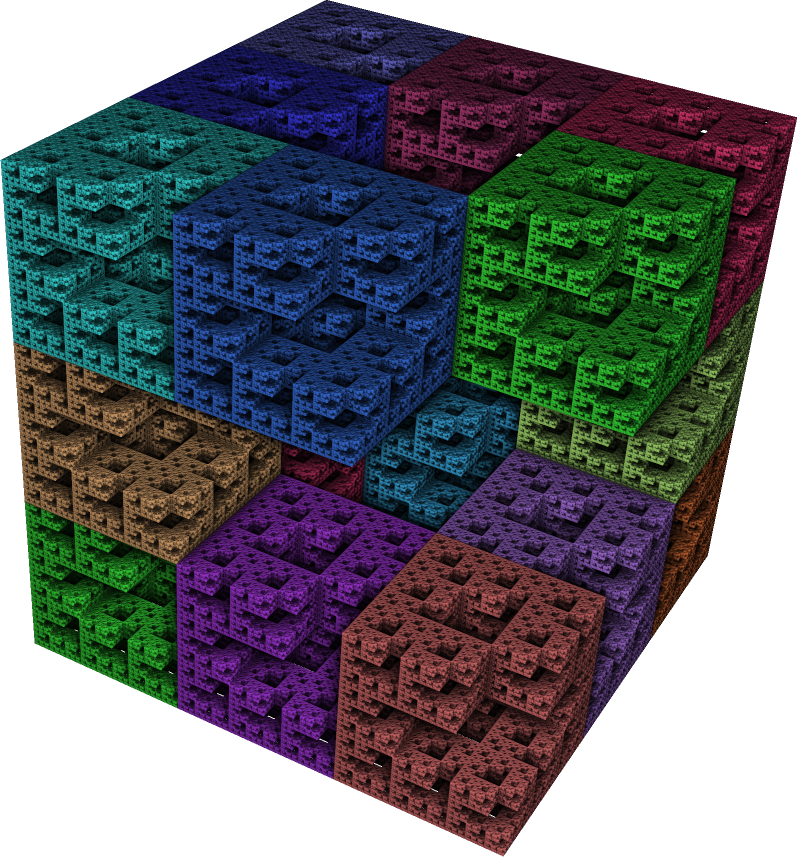
\includegraphics[width=0.45\textwidth]{images/presentation/qK.png}
 \hfill
 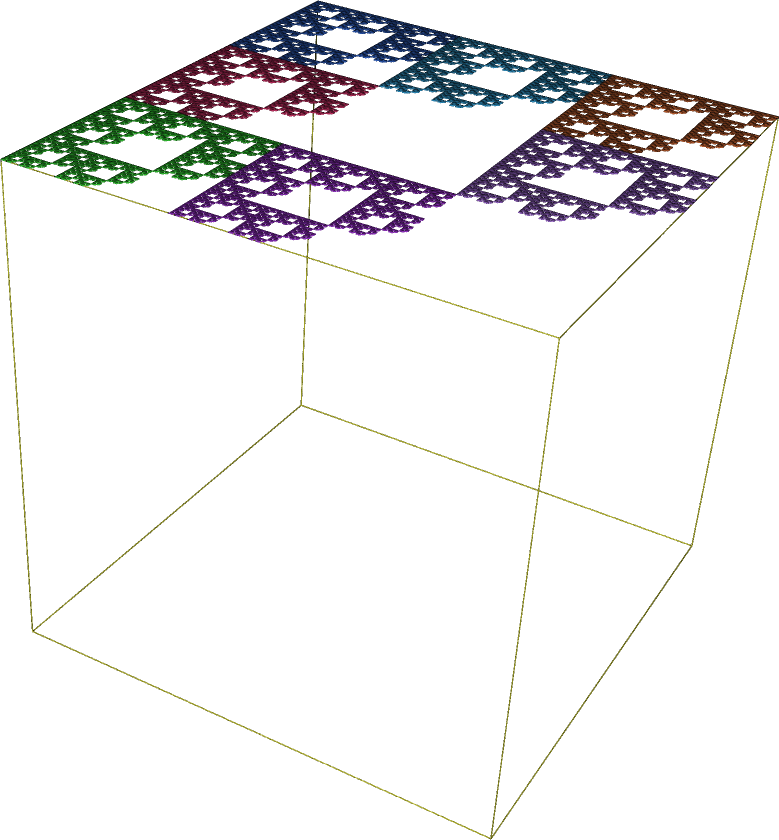
\includegraphics[width=0.45\textwidth]{images/presentation/qK_a.png}
  \caption{Фрактальный куб $K$ и его грань $K_\bma$}
 \label{fig:qK_a}
\end{figure}

\begin{proposition}\label{prop:Ka}
Грань $K_\bma$ фрактального $k$-куба $K$ удовлетворяет уравнению $n K_\bma=K_\bma+D_\bma$, где $D_\bma=D\cap(n-1)P_\bma$.
\end{proposition}

Это утверждение показывает, что каждая грань фрактального $k$-куба сама является фрактальным $k$-кубом.

\begin{proof}
Заметим, что $n K_\bma=n(K\cap P_\bma)=(K+D)\cap nP_\bma.$ 
Если $d\in D$ и   $d\notin(n-1)P_\bma$, то множество $(d+K)\cap nP_\bma$ пусто.
Имеет смысл рассматривать только те $d\in D$, для которых $d\in D\cap (n-1)P_\bma=D_\bma$. Также, если $x\in K\setminus K_\bma$, то $(x+D)\cap nP_\bma=\0$.  
Таким образом, $$n K_\bma=(D+K)\cap n P_\bma=(D_\bma+K)\cap ((n-1)P_\bma+P_\bma)=D_\bma+K_\bma.$$
%Тогда $(d+K)\cap nP_\bma=d+K_\bma$, следовательно $n K_\bma={K_\bma+D_\bma}$.
\end{proof}

\subsection{Пересечения $F_\al$ граней фрактальных $k$-кубов}

Пусть в дальнейшем $K^1$ и $K^2$ --- фрактальные $k$-кубы порядка $n$ с множествами единиц $D^1$ и $D^2$.

\begin{definition}\label{def:F_alpha}
%Пусть даны фрактальные $k$-кубы $K^1$ и $K^2$.
Для любого $\bma\in A$ символом $F_\bma$ обозначим пересечение $K^1_\bma\cap(K^2_{-\bma}+\bma)$ пары граней фрактальных $k$-кубов $K^1$ и $K^2$.
\end{definition}

%Рассмотрим случай, когда $K=K^1=K^2$.
%Тогда $F_\bma$ есть пересечение $K_\bma\cap(K_{-\bma}+\bma)$ пары противоположных граней фрактального $k$-куба $K$.
%В этом случае справедливо следующее предложение.
%
%\begin{proposition}\label{fbma}
%Пусть $K$ --- фрактальный $k$-куб.
%\begin{itemize}[nolistsep]
%\item[1.] Для любого $\bma\in A$ имеет место равенство $K\cap(K+\bma)=F_\bma=F_{-\bma}+\bma $;
%\item[2.] Если $\bi,\bj \in I^k$, $\bi\neq \bj$ и $K_\bi\cap K_\bj\neq\0$, то $d_\bi-d_\bj=\bma$ для некоторого $\bma\in A$, и при этом 
%$$K_\bi\cap K_\bj=\dfrac{d_\bi+F_\bma}{n^k}.$$
%\end{itemize}
%\end{proposition}
%
%\begin{proof}
%1. Поскольку $P\cap (P+\bma)=P_\bma=P_{-\bma}+\bma$, то мы имеем цепочку равенств 
%$$K\cap(K+\bma)= K_\bma\cap (K_{-\bma}+\bma)=F_\bma=F_{-\bma}+\bma.$$
%
%2. Заметим, что $S_\bi^{-1}(K_\bi\cap K_\bj)=K\cap S_\bi^{-1}(K_\bj)=K\cap (K+d_\bj-d_\bi)$. 
%Так как $d_\bj-d_\bi\in\zz^k$, последнее пересечение может быть непусто только в том случае, если $d_\bj-d_\bi$ равно некоторому $\bma\in A$. 
%В этом случае $K\cap(K+d_\bj-d_\bi)=F_\bma$.
%Значит $K_\bi\cap K_\bj= S_\bi(F_\bma)= \dfrac{d_\bi+F_\bma}{n^k}$. 
%\end{proof}
%
%Из предложения \ref{fbma} следует, что для любого фрактального $k$-куба существует $\dfrac{3^k-1}{2}$ способов пересечения смежных копий одинакового размера (поскольку $F_\bma$ и $F_{-\bma}$ соответствуют одному и тому же способу смежности копий). 
%Любое из этих пересечений является образом множества из системы $\{F_\bma\ :\ \bma\in A\mmm\{0\}\}$ относительно некоторого отображения $S_\bi$. 

Из $P\cap (P+\bma)=P_\bma=P_{-\bma}+\bma$ следует, что 
\begin{equation}\label{eq:fbma}
F_{\bma}=K^1_\bma\cap(K^2_{-\bma}+\bma)=K^1\cap(K^2+\bma).
\end{equation}

%При $|\bma|=k$ множество $F_{\bma}=\left(\frac{\al_1+1}{2},\ldots,\frac{\al_k+1}{2}\right)$, если $(n-1)\cdot\left(\frac{\al_1+1}{2},\ldots,\frac{\al_k+1}{2}\right)\in D^1$ и $(n-1)\cdot\left(\frac{-\al_1+1}{2},\ldots,\frac{-\al_k+1}{2}\right)\in D^2$, в противном случае $F_{\bma}=\0$. 
%Иными словами, множества $F_{(\pm1,\ldots,\pm1)}$ соответствуют пересечениям противоположных вершин $k$-куба $P$, а потому являются одноточечными или пустыми.

Уравнения, задающие множества $F_\bma$, получаются из следующей теоремы.

\begin{theorem}\label{IFC}
%Пусть $K^1$ и $K^2$ --- фрактальные $k$-кубы порядка $n$ с множествами единиц $D^1$ и $D^2$.
Семейство множеств $\{F_\bma=K^1\cap(K^2+\bma)\ :\ \bma\in A\}$ удовлетворяет системе уравнений 
\begin{equation}\label{sideint}
%\left\{
F_\bma=\bigcup\limits_{\bmb\sqsupseteq\bma} 
\dfrac{F_\bmb+G_{\bma\bmb}}{n},
%\ \text{ где } \bma\in A,
%\right\}
\end{equation}
где $G_{\bma\bmb}=D^1\cap(D^2+n\bma-\bmb)$.
\end{theorem}

Множество $G_{\bma\bma}=D^1\cap(D^2+(n-1)\bma)$ мы для удобства обозначим как $G_{\bma}$.

\begin{proof}
%Поскольку $P\cap (P+\bma)=P_\bma=P_{-\bma}+\bma$, то справедлива цепочка равенств
Справедлива цепочка равенств
\begin{equation}\label{line}
\begin{split}
nF_\bma &= nK^1\cap(nK^2+n\bma)=(K^1+D^1)\cap(K^2+D^2+n\bma)=\\
        &= \bigcup\limits_{d_1\in D^1,\ d_2\in D^2}(K^1+d_1)\cap (K^2+d_2+n\bma).
\end{split}
\end{equation}

Из соотношения $(K^1+d_1)\cap (K^2+d_2+n\bma)\neq\0$ следует, что \\
$d_2-d_1+n\bma=\bmb$ для некоторого $\bmb\in A$.

Рассматривая $i$-ю координату в последнем равенстве, мы получаем
$$d_{2i}-d_{1i}+n\al_i=\be_i.$$ 
Из того, что $\al_i,\be_i\in\{-1,0,1\}$ и $|d_{2i}-d_{1i}|\le n-1$, вытекают следующие утверждения.

\begin{itemize}[nolistsep]
 \item[(i)] Если $\al_i=1$, то $\be_i>0$, а значит, $\be_i=\al_i$ и $d_{2i}-d_{1i}=n-1$.
 \item[(ii)] Если $\al_i=-1$ , то $\be_i<0$, поэтому $\be_i=\al_i$ и $d_{2i}-d_{1i}=1-n$.
 \item[(iii)] Если $\al_i=0$ то $d_{2i}-d_{1i}=\be_i\in\{-1,0,1\}$.
\end{itemize} 
\medskip

Из утверждений (i), (ii) и (iii) следует что $\bmb\sqsupseteq\bma$.

Равенство $d_1=d_2+n\bma-\bmb$ показывает, что $d_1$ принадлежит множеству $D^1\cap(D^2+n\bma-\bmb)=D^1_\bma\cap(D^2_{-\bma}+n\bma-\bmb)$, которое мы обозначили как $G_{\bma\bmb}$.
Каждое $d_1\in G_{\bma\bmb}$ задаёт единственное $d_2$ и для них справедливы равенства 
$$(K^1+d_1)\cap (K^2+d_2+n\bma)= (K^1\cap(K^2+\bmb))+d_1= F_\bmb+d_1.$$ 
Возьмём объединение по всем $d_1\in G_{\bma\bmb}$, тогда равенство \eqref{line} превратится в $$nF_\bma= \bigcup\limits_{\bmb\sqsupseteq\bma} (F_\bmb+G_{\bma\bmb}).$$
\end{proof}

%\begin{theorem}\label{IFC}
%Семейство $\{F_\bma, \bma\in A_k\}$ пересечений $F_\bma =K_{1}\cap (K_{2}+\bma)$ удовлетворяет системе $\Sa$ уравнеий
% 
%\begin{equation}\label{perall}
%F_\bma=\bigcup\limits_{\bmb\sqsupseteq{\bma}}T_{\bma\bmb}(F_\bmb),\qquad \bma\in A_k,
%\end{equation}
% 
%где для каждого $\bmb\sqsupseteq\bma$, 
%\begin{equation}\label{Gab}
%T_{\bma\bmb}(F_\bmb)=\frac{1}{n}(F_\bmb+G_{\bma\bmb})\mbox{\quad  \text{и} \quad}
%  G_{\bma\bmb}=D_1\cap(D_2+n\bma-\bmb)
%\end{equation}
%\end{theorem}

%\begin{proof}
%Представим $F_\bma$ как $K_1\cap (K_2+\bma)=\dfrac{1}{n}\bigl((K_1+D_1)\cap (K_2+D_2+n\bma)\bigr).$ \\
%
%Пусть $d_1\in D_1$ и $d_2\in D_2$, тогда пересечение $(K_{1}+d_1)\cap (K_{2}+d_2+n\bma)$ непусто если $(P+d_1)\cap (P+d_2+n\bma)\neq\0$, что означает, что вектор $\bmb=d_2-d_1+n\bma$ лежит в множестве $A$. 
%Поскольку для любого номера координаты $i=1,\ldots  ,k$ мы имеем $|(d_2-d_1)_i|\le n-1$, это возможно только если $\bmb\sqsupseteq \bma$.\\
%
%Если $\bmb=\bma$, то $d_1=d_2+(n-1)\bma$, следовательно $d_1\in D_1\cap(D_2+(n-1)\bma)= G_\bma$.
%
%Если $\bmb\sqsupset\bma$, то $(K_{1}+d_1)\cap (K_{2}+d_2+n\bma)=(K_1\cap (K_2+\bmb))+d_1$, и $d_1\in D_1\cap(D_2+n\bma-\bmb)$. Множество $D_1\cap(D_2+n\bma-\bmb)$ мы обозначим как  $G_{\bma\bmb}$. 
%
%Заметим, что  $G_{\bma\bma}=D_1\cap(D_2+n\bma-\bma)$, а значит $G_{\bma\bma}=G_{\bma}$.
%
%В результате мы получаем  $F_\bma=\frac{1}{n}\bigcup\limits_{\bmb\sqsupseteq{\bma}}(F_\bmb+G_{\bma\bmb})=
%\frac{1}{n}(F_\bma+G_\bma)\cup\bigcup\limits_{\bmb\sqsupset{\bma}}\frac{1}{n}(F_\bmb+G_{\bma\bmb})$.
%\end{proof}

Из теоремы \ref{IFC} и замечания \ref{rmk:point} следует, что при $|\bma|=k$ множество $F_\bma$ не более чем одноточечно.
Говоря конкретнее, $F_\bma=\left\{\left(\frac{\al_1+1}{2},\ldots, \frac{\al_k+1}{2}\right)\right\}$ тогда и только тогда, когда $G_\bma=\left\{(n-1)\cdot\left(\frac{\al_1+1}{2},\ldots, \frac{\al_k+1}{2}\right)\right\}$.\\

Множество $F_\bma$ пусто, если $G_\bma=\0$ и для любого $\bmb\sqsupset\bma$ множество $F_\bmb+G_{\bma\bmb}=\0$.
Это позволяет вывести условие того, что $F_\bma$ пусто.

\begin{lemma}
Множество $F_\bma=\0$ тогда и только тогда, когда для любого $\bmb\sqsupseteq\bma$ и для любой конечной последовательности\\ $\bma=\bma_0\sqsubseteq\bma_1\sqsubseteq\ldots \bma_{p-1}\sqsubseteq\bma_p=\bmb$ произведение 
$\#G_{\bma_0\bma_1}\#G_{\bma_1\bma_2}\ldots  \#G_{\bma_{p-1}\bma_p}\#G_{\bmb}$ равно нулю. 
\qed
\end{lemma} 

Отношения между множествами $F_\bma$, установленные в Теореме \ref{IFC}, приводят к {\em структурному графу $\Ga_\Sa$} системы $\Sa$. 

\begin{definition}
Структурным графом $\Ga_\Sa$ называется отмеченный ориентированный граф с множеством вершин $\{\bma\in A\ :\ F_\bma\neq\0\}$ и множеством рёбер $\{(\bma, \bmb)\ :\ \bma\sqsubseteq\bmb, G_{\bma\bmb}\neq\0, F_\bmb\neq\0\}$, где ребро $(\bma, \bmb)$ направлено из $\bma$ в $\bmb$ и отмечено $G_{\bma\bmb}$.
\end{definition}

\begin{figure}[h!]
    \centering
    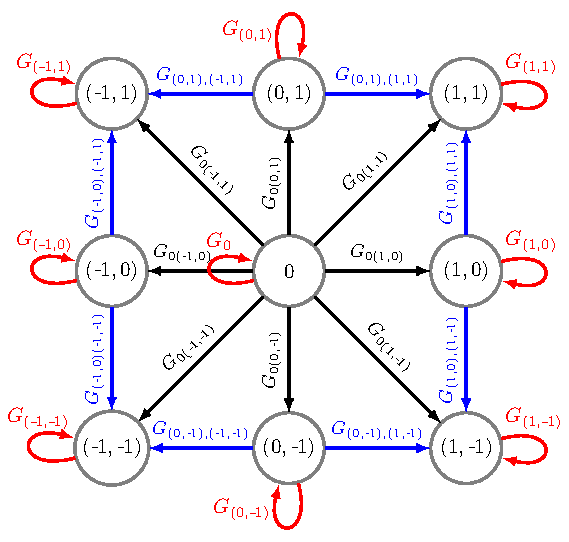
\includegraphics[width=.6\textwidth]{structure_graph_full_new.pdf}
    \caption{Структурный граф $\Ga_\Sa$ в общем случае для пересечения двух фрактальных квадратов}
\end{figure}

В общем случае граф $\Ga_\Sa$ содержит $3^k$ вершин и $5^k$ ребер, при этом $3^k$ ребер являются петлями.

%Структурный граф $\Ga_\Sa$ можно упростить без потери информации об отношениях между множествами $F_\bma$.
%Для этого требуется удалить из графа вершины, которым соответсвуют пустые $F_\bma$, а также удалить те рёбра $(F_\bma,F_\bmb)$ при $\bmb\sqsupseteq\bma$, для которых $G_{\bma\bmb}=\0$ или $F_\bmb=\0$.
%После такого упрощения структурный граф для системы $\Sa$, определенной в теореме \ref{IFC}, имеет множество вершин $V_\Sa=\{F_\bma: \bma\in A, F_\bma\neq\0\}$ и множество ребер $E_\Sa=\{(F_\bma, F_\bmb): \bma\sqsupseteqeq\bmb, G_{\bma\bmb}\neq\0, F_\bmb\neq\0\}$.




\begin{definition}
Мы говорим, что в граф $\Ga_\Sa$  содержит  {\em направленный путь от $\bma$ до $\bmb$}, если 
\begin{itemize}[nolistsep]
\item[1.] $\bma\sqsubset\bmb$ и существует последовательность $\bma=\bma_0\sqsubset\bma_1\sqsubset\ldots\sqsubset\bma_{p-1}\sqsubset\bma_p=\bmb$ такая, что для любых  $j=0, \ldots, p$ множества $F_{\bma_j}\neq\0$  и  $G_{\bma_{j-1}\bma_j}\neq\0$ для $j=1, \ldots, p$; либо
\item[2.] $\bma=\bmb$ и  $G_{\bma}\neq\0$.
\end{itemize}
Мы пишем $\bmb\succcurlyeq\bma$, если  $\Ga_\Sa$ содержит направленный путь от $F_\bma$ до $F_\bmb$, и $\bmb\succ\bma$, если при этом $\bma\neq\bmb$.
\end{definition}
 
%Если $\bmb\succcurlyeq\bma$ или $\bma\succcurlyeq\bmb$, то мы говорим, что $\bma$ и $\bmb$ являются $\Ga${\em-сравнимы}.
Мы обозначим через $\Ga_\bma$ подграф в $\Ga_\Sa$, все вершины которого являются $\bmb$ такими, что $\bmb\succcurlyeq\bma$. 
Если структурный граф $\Ga_\Sa$ несвязен, то $\Ga_0$ --- это та компонента графа $\Ga_\Sa$, которая содержит вершину $0$.\\
Мы говорим, что $\bmb$ является {\em максимальным} для $\Ga_\bma$, если $\bmb$ является единственной вершиной в $\Ga_\bmb$.
Мы говорим, что $\bmb$ является {\em минимальным} для $\Ga_\bma$, если в $\Ga_\bma$ нет $\bma$ такого, что $\bma\prec\bmb$.

Исходя из теоремы \ref{IFC}, граф $\Ga_\bma$ показывает множество всех уравнений, которые полностью определяют каждое из множеств $F_\bmb$, для которых $\bmb\succcurlyeq\bma$.


%\subsection{Мощность пересечений копий фрактального квадрата}
%
%Рассмотрим фрактальный квадрат $K=\dfrac{K+D}{n}$ и пару таких копий $\dfrac{K+d_1}{n}$ и $\dfrac{K+d_2}{n}$, что $d_2=d_1+\bma$, где $\bma\in A\mmm\{0\}$.
%Назовём такую пару копий {\em копиями с $\bma$-соседством}.
%Тогда $\dfrac{K+d_1}{n}\cap\dfrac{K+d_2}{n}=\dfrac{d_1+F_\bma}{n}$, значит мощность пересечения копий с $\bma$-соседством совпадает с мощностью множества $F_\bma$.
%Уравнение \eqref{sideint} в Теореме \ref{IFC} позволяет нам оценить мощность множества $F_\bma$.
%
%\begin{theorem}\label{fin_int}
%Пусть $K=\dfrac{K+D}{n}$ --- фрактальный квадрат. Рассмотрим $F_\bma, \bma\in A\mmm\{0\}$.
%\begin{itemize}[nolistsep]
% \item[(i)] Если $\#G_{\bma\bma}> 1$, то множество $F_\bma$ несчётно.
% \item[(ii)] Если $\#G_{\bma\bma}=1$ и существует $\bmb\sqsupset\bma$ такое, что  $F_\bmb$ непусто и $\#G_{\bma\bmb}\geq1$, то $F_\bma$ бесконечное счётное.
% \item[(iii)] Множество $F_\bma$ конечно в следующих случаях:
% \begin{itemize}[nolistsep]
% \item[\textbf{(a)}] $\#G_{\bma\bma}=1$ и $\#F_\bmb\cdot\#G_{\bma\bmb}=0$ для каждого $\bmb\sqsupset\bma$;
% \item[\textbf{(b)}] $\#G_{\bma\bma}=0$ и существует $\bmb\sqsupset\bma$ такое, что $\#F_\bmb\cdot\#G_{\bma\bmb}\geq1$.
% \end{itemize}
%\end{itemize} 
%\end{theorem}
%
%\begin{proof}
%При $\bma\in A\mmm\{0\}$ множество $F_\bma$ удовлетворяет уравнению
%$F_\bma=\bigcup\limits_{\bmb\sqsupseteq\bma} \dfrac{F_\bmb+G_{\bma\bmb}}{n}$, 
%где $G_{\bma\bmb}=D_\bma\cap(D_{-\bma}+n\bma-\bmb)$.\\
%Если $\bma\in\{(1,0),\ (-1,0),\ (0,1),\ (0,-1)\}$, то $\#\{\bmb:\bmb\sqsupset\bma\}=2$, при этом $\bmb\in\{(1,1),\ (-1,1),\ (1,-1),\ (-1,-1)\}$.\\
%Если $\bma\in\{(1,1),\ (-1,1),\ (1,-1),\ (-1,-1)\}$, то $\#\{\bmb:\bmb\sqsupset\bma\}=0$.\\
%
%Для $\bma\in\{(1,1),\ (-1,1),\ (1,-1),\ (-1,-1)\}$, то $\#G_{\bma\bmb}\leq1$ множество $F_\bma$ не более чем одноточечно.\\
%
%Далее предполагаем, что $\bma\in\{(1,0), (-1,0), (0,1), (0,-1)\}$.\\
%
%(i) Если $\#G_{\bma\bma}> 1$, то $F_\bma$ содержит в себе фрактальный квадрат с множеством единиц $G_{\bma\bma}$, который имеет мощность континуума.\\
%
%(ii) Рассмотрим случай, когда $\#G_{\bma\bma}=1$ и существует $\bmb\sqsupset\bma$ такое, что  $F_\bmb$ непусто и $\#G_{\bma\bmb}\geq1$. 
%Такое непустое $F_\bmb$ единственно, поскольку иначе $\#G_{\bma\bma}>1$.
%Множество $\dfrac{F_\bmb+G_{\bma\bmb}}{n}$ конечно, поэтому $F_\bma=\bigcup\limits_{n=1}^\8 S_\bma^n$.\\
%
%(iii.{\bf a}) Пусть $G_{\bma\bma}=\{d_i\}$ и $\#F_\bmb\cdot\#G_{\bma\bmb}=0$ для каждого $\bmb\sqsupset\bma$.
%В этом случае из равенства $F_\bma=\dfrac{F_\bma+\{d_i\}}{n}$следует $F_\bma=\left\{\dfrac{d_i}{n-1}\right\}$.\\
%
%(iii.{\bf b}) Наконец, рассмотрим случай, когда $G_{\bma\bma}=\0$ и существует $\bmb\sqsupset\bma$ такое, что $\#F_\bmb\cdot\#G_{\bma\bmb}\geq1$.
%При $G_{\bma\bma}=\0$ может существовать не более одного $\bmb\sqsupset\bma$ такого, что $F_\bmb\neq\0$, в противном случае $\#G_{\bma\bma}\geq2$.
%Так как $\#F_\bmb=1$, множество $F_\bma=\dfrac{F_\bmb+G_{\bma\bmb}}{n}$ конечно, а говоря точнее, $\#F_\bma=\#G_{\bma\bmb}$.
%\end{proof}
%
%Далее докажем, что фрактальный квадрат, являющийся дендритом, обладает свойством одноточечного пересечения.
%Поэтому укажем условия, при которых $F_\bma$ одноточечно:
%
%\begin{corollary}\label{onepoint} 
%Множество $F_\bma$ одноточечно, если \\
%\textbf{(a)} $\#G_{\bma\bma}=1$ и $\#F_\bmb\cdot\#G_{\bma\bmb}=0$ для каждого $\bmb\sqsupset\bma$; или\\
%\textbf{(b)} $\#G_{\bma\bma}=0$ и существует $\bmb\sqsupset\bma$ такое, что $\#F_\bmb\cdot\#G_{\bma\bmb}=1$.
%\hfill\qed
%\end{corollary}

\subsection{Мощность множества $F_\al$}

Рассмотрим фрактальные $k$-кубы $K^1=\dfrac{K^1+D^1}{n}$ и  $K^2=\dfrac{K^2+D^2}{n}$, и пару таких копий $\dfrac{K^1+d_1}{n}\in K^1$ и $\dfrac{K^2+d_2}{n}\in K^2$, что $d_2=d_1+\bma$, где $\bma\in A$.
Назовём такую пару копий {\em копиями с $\bma$-соседством}.
Тогда $\dfrac{K^1+d_1}{n}\cap\dfrac{K^1+d_2}{n}=\dfrac{d_1+F_\bma}{n}$, поэтому мощность пересечения копий с $\bma$-соседством совпадает с мощностью множества $F_\bma$.
Уравнение \eqref{sideint} в Теореме \ref{IFC} позволяет нам оценить мощность множества $F_\bma$.

\begin{theorem}\label{fin_int}
\qquad
%Пусть $K^1=\dfrac{K^1+D^1}{n}$ и $K^2=\dfrac{K^2+D^2}{n}$ --- фрактальные $k$-кубы. 
%Рассмотрим $F_\bma=K^1\cap(K^2+\bma)$, где $\bma\in A$.
\begin{enumerate}[nolistsep]
\item[(1)] Если $\#G_\bmb>1$ для некоторого $\bmb\succcurlyeq\bma$, то  $F_\bma$ несчетно.

\item[(2a)] Если  $\#G_\bmb\leq1$ для любого $\bmb\succcurlyeq\bma$, то  $F_\bma$ не более чем счетно.


\item[(2b)] Если при этом существует $\bmb'\succ\bmb$ такое, что $\#G_\bmb=1$ и $F_{\bmb'}\neq\0$, то $F_\bma$ счетно.

\item[(3)] Если  $\#G_\bmb=1$ для всех максимальных вершин $\bmb$ в $\Gamma_\bma$, и $G_{\bma_i}=\0$ для всех остальных вершин $\bma_i$ в $\Gamma_\bma$, то $F_\bma$ конечно.
В этом случае $\#F_\bma$ не превосходит сумму   композиций $\prod \limits_{j=1}^{p-1}\# G_{\bma_j\bma_{j+1}}$, взятых по всем цепочкам $\bma=\bma_1\prec\ldots\prec\bma_p=\bmb$, где $\bmb$  максимален в $\Gamma_\bma$.

\item[(4)] Если все $\bma_i\succcurlyeq\bma$ образуют единственную цепочку $\bma=\bma_1\prec\ldots\prec\bma_p$, в которой  $\# G_{\bma_j\bma_{j+1}}=1$, $G_{\bma_j}=\0$ и $\#G_{\bma_p}=1$ для всех $j\le p-1$, то  $\#F_\bma=1$.
\end{enumerate}
\end{theorem}


\begin{proof}
Введём для $\bmb\sqsupseteq\bma$ обозначение $T_{\bma\bmb}(x) = \dfrac{x+G_{\bma\bmb}}{n}$.
Тогда формула \eqref{sideint} представима в виде 
$$F_{\bma} = T_{\bma\bma}(F_\bma) \cup \bigcup_{\bmb\sqsupset\bma}T_{\bma\bmb}(F_\bmb).$$

(1) 
Если $\#G_{\bmb}> 1$, то $F_\bmb$ содержит в себе фрактальный $k$-куб с множеством единиц $G_{\bmb}$, а значит, $F_\bmb$ имеет мощность континуума.
Тогда множество $F_\bma$ либо совпадает с несчётным $F_\bmb$ (при $\bmb=\bma$), либо содержит в себе его образ относительно  некоторой гомотетии (при $\bmb\succ\bma$).\\
%существует такая цепочка $\bma = \bma_1\sqsubset \ldots \sqsubset\bma_p = \bmb$, что $\prod \limits_{j=1}^{p-1}\# G_{\bma_j\bma_{j+1}}\geq1$.
%Этой цепочке соответсвует композиция $T_{\bma_1\bma_2} \circ \ldots \circ  T_{\bma_{p-1}\bma_p}$.
%$T_{\bma_1\bma_2} \circ \ldots \circ  T_{\bma_{p-1}\bma_p} (F_\bmb)$


(2)
Обозначим $B=\bigcup\limits_{\bma\sqsupset0}\dfrac{G_{0\bma}+F_\bma}{n}$.
Тогда $F_0 = \dfrac{G_0+F_0}{n}\cup B$.
Пусть $B$ не пусто и не более чем счётно.
Тогда при $G_0=\0$ имеем $F_0=B$.
При $G_0=\{d_0\}$ верны равенства 
$$F_0 = \dfrac{d_0+F_0}{n}\cup B = \dfrac{d_0}{n-1} \cup \bigcup\limits_{m=0}^\8 S^m(B),\ \text{ где }\ S(x)=\dfrac{d_0+x}{n}.$$
Если $B\neq\dfrac{d_0}{n-1}$, то  $F_0$ бесконечно.

Если $\#B=1$, то $B=\dfrac{F_\bma+G_{0\bma}}{n}$, где $\#F_\bma=1$ и $G_{0\bma}=\{d_{0\bma}\}$.
Координаты точки $\dfrac{d_0}{n-1}$ кратны $\dfrac{1}{n-1}$, в то время как координаты точки $B$ --- дроби с $n$ в знаменателе, значит покоординатно $(\dfrac{d_0}{n-1})_i=(\dfrac{F_\bma+G_{0\bma}}{n})_i\in\{0,1\}$.
Это возможно только если $F_\bma = \dfrac{d_\bma+F_\bma}{n}$ и $d_0=d_\bma=d_{0\bma}$.
Из последнего равенства следует, что $\{d_0,\ d_0-(n-1)\bma,\ d_0-n\bma\}\IN D^2$, что возможно только при $\bma=0$.

Для каждого $\bmb\succ0$, максимального в $\Gamma_0$, множество $F_\bmb$ всегда одноточечно.
Индуктивно для каждого $\bma\succ0$ множество $F_\bma$ также не более чем счётно.

(3)
Обозначим множество максимальных вершин в $\Gamma_\bma$ символом $\max\Gamma_\bma=\{\bmb\ :\ \bmb\succcurlyeq\bma \text{ и } \nexists\bmb'\succ\bmb\}$.
Для $\bmb\in\max\Gamma_\bma$ множество $F_\bmb$ одноточечно.
Тогда для любой цепочки $\bma=\bma_1\prec\ldots\prec\bma_p=\bmb$ множество $T_{\bma_1\bma_2} \circ \ldots \circ  T_{\bma_{p-1}\bma_p} (F_\bmb)$ конечно.
При этом для $F_\bma$ справедливо представление
$$F_\bma=\bigcup_{
		\substack{
			\bmb\in\max\Gamma_\bma\\ 
			\bma=\bma_1\prec\ldots\prec\bma_p=\bmb}}
	T_{\bma_1\bma_2} \circ \ldots \circ  T_{\bma_{p-1}\bma_p} (F_\bmb).$$
Следовательно
$$\#F_\bma\leq\sum_{
		\substack{
			\bmb\in\max\Gamma_\bma\\ 
			\bma=\bma_1\prec\ldots\prec\bma_p=\bmb}}
	\#G_{\bma_1\bma_2} \cdot \ldots \cdot  \#G_{\bma_{p-1}\bma_p}.$$
	
(4) Согласно формулировке, имеется единственное $\bmb\in\max\Gamma_\bma$ и единственная цепочка $\bma=\bma_1\prec\ldots\prec\bma_p=\bmb$.
Тогда $F_\bma=T_{\bma_1\bma_2} \circ \ldots \circ  T_{\bma_{p-1}\bma_p} (F_\bmb)$ и $\#F_\bma=\#G_{\bma_1\bma_2} \cdot \ldots \cdot  \#G_{\bma_{p-1}\bma_p}\cdot\#F_\bmb=1.$
\end{proof}


\begin{example}[Пересечение двух фрактальных квадратов, состоящее из $24$ точек, и его стркутурный граф $\Ga_\Sa$] \label{ex:3_1}

Рассмотрим пересечение фрактальных квадратов $K_1$ и $K_2$ порядка $6$ с множествами единиц $D_1$ и $D_2$.
На рисунке \ref{fig:FSI_6x6_DSK} слева мы представляем $D_1$ и $D_2$ множеством красных квадратов $T_1(P)=\dfrac{D_1+P}{6}$ и синих квадратов $T_2(P)=\dfrac{D_2+P}{6}$.
На этом же рисунке справа показаны фрактальные квадраты $K_1$ и $K_2$. \\

Большинство из множеств $G_\bma$, а именно, 
$G_0$, $G_{(1,0)}$, $G_{(-1,0)}$, $G_{(0,1)}$, $G_{(0,-1)}$, $G_{(1,1)}$, $G_{(1,-1)}$ и $G_{(-1,1)}$ являются пустыми, и только $G_{(-1,-1)}=\{(0,0)\}$. 
Следовательно, $F_{(1,1)}=F_{(1,-1)}=F_{(-1,1)}=\0$ и $F_{(-1,-1)}=\{(0,0)\}$.

\begin{figure}[H]
    \centering
    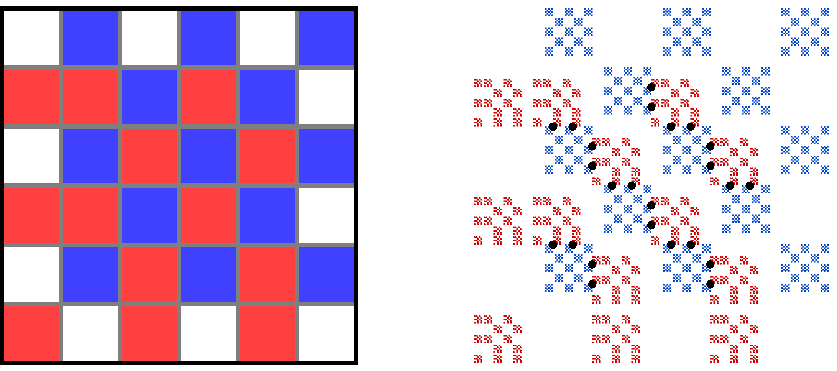
\includegraphics[width=0.8\textwidth]{FSI_6x6_DS_new.pdf}
    \caption{Множества $\dfrac{D_1+P}{6}$ и $\dfrac{D_2+P}{6}$ (слева) и фрактальные квадраты $K_1$ и $K_2$ (справа). $K_1$ и $K_2$ пересекаются по чёрным точкам}
    \label{fig:FSI_6x6_DSK}
\end{figure}

Множество $F_{(1,0)}$ пусто, поскольку $G_{(1,0)}$, $F_{(1,1)}$ и $F_{(1,-1)}$ пусты. 
По той же причине $F_{(0,1)}=\0$.

Тут $G_{0(-1,0)}=\{(1,2), (1,4),(2,3), (3,2), (3,4), (4,3)\}$ и $G_{(-1,0)(-1,-1)}=\{(0,2), (0,4)\}$.
Аналогичным образом $\#G_{(0,-1)(-1,-1)}=2$ и $\#G_{0(0,-1)}=6$.

Таким образом, после удаления пустых вершин и ребер
граф $\Ga_\Sa$ содержит четыре вершины  $F_0$, $F_{(-1,0)}$, $F_{(0,-1)}$, $F_{(-1,-1)}$ и четыре ребра, которым соответствуют $G_{(-1,0)(-1,-1)}$, $ G_{(0,-1)(-1,-1)}$, $G_{0(-1,0)}$ и $G_{0(0,-1)}$.

Из теоремы \eqref{fin_int} следует, что
$\#F_{(-1,0)}=\#F_{(0,-1)}=2$ и $\#F_0=\#F_{(-1,0)}\cdot\#G_{0(-1,0)}+\#F_{(0,-1)}\cdot\#G_{0(0,-1)}=24.$

\begin{figure}[H]
    \centering
    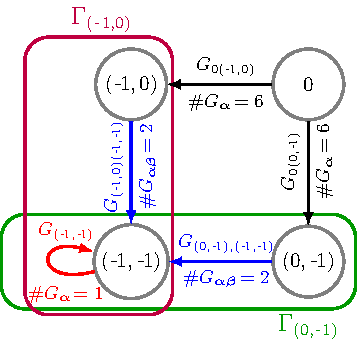
\includegraphics[width=.45\textwidth]{FSI_6x6_SG_new.pdf}
    \caption{Cтруктурный граф $\Ga_\Sa=\Ga_0$ и его подграфы $\Ga_{(0,-1)}$ и $\Ga_{(-1,0)}$}
\end{figure} 
\end{example} 




\section{Фрактальный куб с одноточечным пересечением, являющийся дендритом}

Далее будут получены условия, при которых фрактальный $k$-куб с одноточечным пересечением является дендритом.

\subsection{Свойство одноточечного пересечения}

Далее будем полагать, что $K=K^1=K^2$.
Тогда $F_\bma$ есть пересечение $K_\bma\cap(K_{-\bma}+\bma)$ пары противоположных граней фрактального $k$-куба $K$.
В этом случае справедливо следующее предложение.

\begin{proposition}\label{fbma}
Пусть $K$ --- фрактальный $k$-куб.
\begin{itemize}[nolistsep]
\item[1.] Для любого $\bma\in A$ имеет место равенство $K\cap(K+\bma)=F_\bma=F_{-\bma}+\bma $;
\item[2.] Если $\bi,\bj \in I^k$, $\bi\neq \bj$ и $K_\bi\cap K_\bj\neq\0$, то $d_\bi-d_\bj=\bma$ для некоторого $\bma\in A$, и при этом 
$$K_\bi\cap K_\bj=\dfrac{d_\bi+F_\bma}{n^k}.$$
\end{itemize}
\end{proposition}

\begin{proof}
1. Поскольку $P\cap (P+\bma)=P_\bma=P_{-\bma}+\bma$, то мы имеем цепочку равенств 
$$K\cap(K+\bma)= K_\bma\cap (K_{-\bma}+\bma)=F_\bma=F_{-\bma}+\bma.$$

2. Заметим, что $S_\bi^{-1}(K_\bi\cap K_\bj)=K\cap S_\bi^{-1}(K_\bj)=K\cap (K+d_\bj-d_\bi)$. 
Так как $d_\bj-d_\bi\in\zz^k$, последнее пересечение может быть непусто только в том случае, если $d_\bj-d_\bi$ равно некоторому $\bma\in A$. 
В этом случае $K\cap(K+d_\bj-d_\bi)=F_\bma$.
Значит $K_\bi\cap K_\bj= S_\bi(F_\bma)= \dfrac{d_\bi+F_\bma}{n^k}$. 
\end{proof}

Из предложения \ref{fbma} следует, что для любого фрактального $k$-куба существует $\dfrac{3^k-1}{2}$ способов пересечения смежных копий одинакового размера (поскольку $F_\bma$ и $F_{-\bma}$ соответствуют одному и тому же способу смежности копий). 
Любое из этих пересечений является образом множества из системы $\{F_\bma\ :\ \bma\in A\mmm\{0\}\}$ относительно некоторого отображения $S_\bi$. 
Для $\bma\in A$ пара копий $K_{(d)}=\dfrac{K+d}{n}$ и $K_{(d+\bma)}=\dfrac{K+(d+\bma)}{n}$ пересекается по множеству $\dfrac{F_\bma+d}{n}$.
Критическим множеством $\eC=\bigcup\limits_{\bma\sqsupset0}\dfrac{G_{0\bma}+F_\bma}{n}$.

Теорема \ref{fin_int} (4) даёт условия, при которых $F_\bma$ одноточечно.
Это позволяет определить, является ли фрактальный $k$-куб $K$ множеством с одноточечным пересечением. 

\begin{corollary}\label{SIPQ}
%Фрактальный куб $K$ обладает свойством одноточечного пересечения, если структурный граф $\Gamma_\Sa$ представляет собой объединение цепочек $0\prec\bma_{i1}\prec\ldots\prec\bma_{ip_i}$, для которых все $\bma_{ij}$ различны и таковы, что для всех $i$ верно $\#G_{\bma_{ip_i}}=1$ и для всех $i,j$ таких, что $j\le p_i-1$, верно $\# G_{\bma_{ij}\bma_{i,j+1}}=1$ и $G_{\bma_{ij}}=\0$.
Фрактальный $k$-куб $K$ является множеством с одноточечным пересечением, если для каждого $\bma\succ0$ множество $F_\bma$ одноточечно.
\end{corollary}


Согласно теореме \ref{thm:fpden}, самоподобное множество с одноточечным пересечением является дендритом, если его двудольный граф пересечений $\hat\Gamma$ является деревом.
Построим граф $\hat\Gamma$ для фрактального $k$-куба с одноточечным пересечением.

Во фрактальном $k$-кубе $K$ каждой копии $K_{(d)}$ соответсвует единственное $d\in D$, поэтому в двудольном графе пересечений $\hat\Gamma$ мы можем рассматривать вектора из множества единиц в качестве белых вершин графа $\hat\Gamma$.
Пусть $A_D=\{\bma\in A\mmm\{0\}\ :\ F_\bma\neq\0,\ G_{0\bma}\neq\0\}$.
Тогда для каждого $\bma\in A_D$ каждая пара белых вершин $d,\ d+\bma\in D$ графе $\hat\Gamma$ соединена рёбрами с общей чёрной вершиной (которой которой соответсвует одноточечное множество $K_{(d)}\cap K_{(d+\bma)}$).

Этих действий может быть недостаточно для построения достоверного графа $\hat\Gamma$, поскольку чёрная вершина этого графа может быть соединена рёбрами с тремя и более белыми вершинами.
Это соответсвует трём и более копиям фрактального $k$-куба, имеющим общую точку.
На рисунке \ref{fig:triple} выделены две тройки копий во фрактальном квадрате с одноточечным.
У одной тройки копий есть общая точка, поэтому эти копии не образуют цикл в графе $\hat\Gamma$.
Вторая тройка копий образует цикл в графе $\hat\Gamma$, поскольку попарно копии друг с другом пересекаются, но все три копии не имеет общей точки.
Проверить тройку копий фрактального $k$-куба с одноточечным пересечением на наличие общей точки позволяет следующая теорема.


\begin{theorem}\label{thm:triple}
Пусть $K=\dfrac{K+D}{n}$ фрактальный куб с одноточечным пересечением. 

Если существуют неравные $\bma,\bmb\neq0$ такие, что $F_\bma=F_\bmb\neq\0$ и $G_{0\bma}\neq0,\ G_{0\bmb}\neq0$,  то для каждой тройки $d, d+\bma, d+\bmb\in D$ копии $K_{(d)},$ $K_{(d+\bma)}$ и $K_{(d+\bmb)}$ пересекаются по общей точке $\{x\}=\dfrac{F_\bma+d}{n}=\dfrac{F_\bmb+d}{n}$.
\end{theorem}

\begin{proof}
Очевидно, что $K_{(d)}\cap K_{(d+\bma)}=\dfrac{F_\bma+d}{n}$ и $K_{(d)}\cap K_{(d+\bmb)}=\dfrac{F_\bmb+d}{n}$.
Из равенства $F_\bma=F_\bmb$ следует, что
$$K_{(d)}\cap K_{(d+\bma)}=K_{(d)}\cap K_{(d+\bmb)}=\dfrac{F_\bmb+d}{n}=\dfrac{F_\bma+d}{n}=\{x\},$$
то есть $K_{(d)}\cap K_{(d+\bma)}\cap K_{(d+\bmb)}=\{x\}.$

Значит, в двудольном графе пересечений $\hat\Gamma$ белые вершины, соответствующие копиям $K_{(d)}, K_{(d+\bma)}, K_{(d+\bmb)}$, соединены с одной и той же единственной черной вершиной, соответствующей точке $x$.
\end{proof}

\begin{figure}[H]
    \centering
    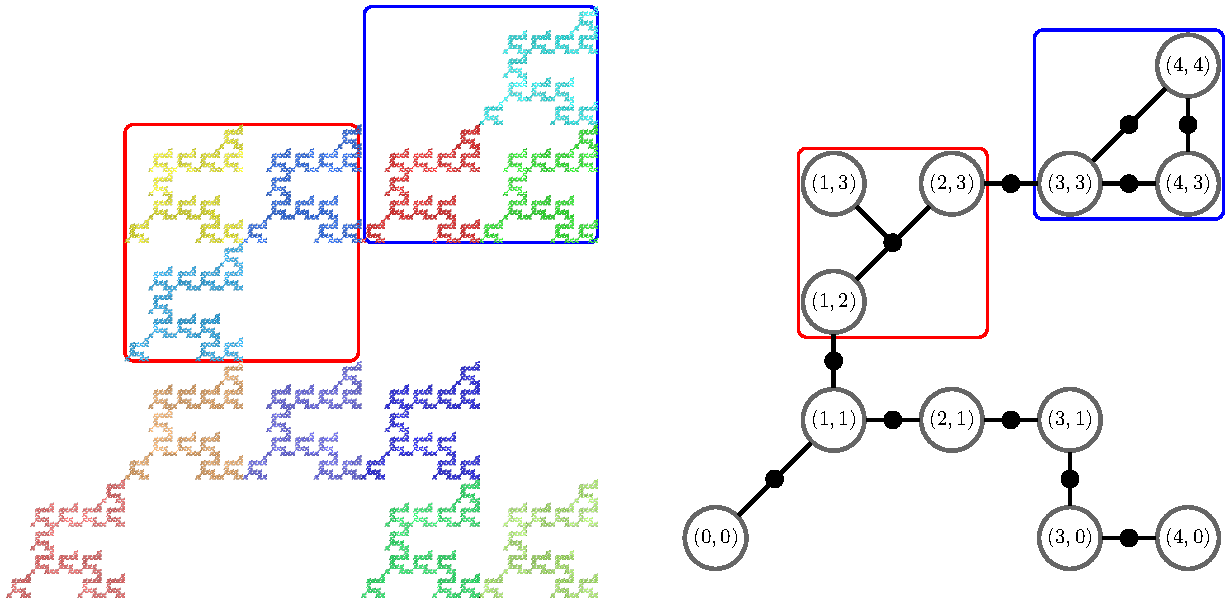
\includegraphics[width=.75\textwidth]{FSD_ord3_SSB.pdf}
    \caption{Тройка копий с общей точкой (обведены красной линией) и тройка копий, образующих в $\hat\Gamma$ цикл (копии обведены синий линией)}
    \label{fig:triple}
\end{figure}

Заметим, что при условиях предыдущей теоремы копии $K_{(d)}, K_{(d-\bma)}, K_{(d-\bmb)}$ попарно пересекаются в трёх различных точках.
$$  K_{(d)}\cap K_{(d-\bma)}=\dfrac{F_\bma+(d-\bma)}{n};\;
    K_{(d)}\cap K_{(d-\bmb)}=\dfrac{F_\bma+(d-\bmb)}{n};$$
$$  K_{(d-\bma)}\cap K_{(d-\bmb)}=\dfrac{F_{\bma-\bmb}+(d-\bma)}{n}=\dfrac{F_{\bmb-\bma}+(d-\bmb)}{n}.$$
Следовательно, белые вершины, соответствующие $K_{(d)}, K_{(d-\bma)}, K_{(d-\bmb)}$, образуют в $\hat\Gamma$ цикл, состоящий из трёх белых и трёх черных точек.

Копии в тройках $\{K_{(d)}, K_{(d-\bma)}, K_{(d+\bmb)\}}$ и $\{K_{(d)}, K_{(d+\bma)}, K_{(d-\bmb)\}}$ также попарно пересекаются по разным множествам или вовсе не пересекаются.

Торема \ref{thm:triple} естественным образом обобщается для случая, в котором $m$ копий имеют общую точку.

\begin{corollary}\label{mpoint}
Пусть $ B=\{d_1,...,d_m\}$ --- такое подможество в $D$, что для любых $d_i,d_j,d_k\in B$ справедливо 
$$(d_j-d_i),(d_k-d_i)\in A\setminus0\text{ и } F_{d_j-d_i}=F_{d_k-d_i}\neq\0.$$
Тогда существует такая точка $x\in K$, что для любых $d_i,d_j\in B$ справедливо равенство $K_{(d_i)}\cap K_{(d_j)}=\{x\}$, а $x$ соответсвует чёрной вершине порядка $m$ в графе $\hat\Gamma$.
\qed
\end{corollary}



\subsection{Алгоритм проверки фрактального $k$-куба}

Чтобы проверить, является ли фрактальный $k$-куб $K$ дендритом с одноточечным пересечением, нужно выполнить следующие шаги:

\begin{enumerate}

\item Cогласно теореме \ref{IFC}, найдём все множества $G_\bma, G_{\bma\bmb}$ и выразим систему $\Sigma=\{F_\bma=K\cap(K+\bma)\ :\ \bma\in A\}$.

\item Построим для системы $\Sa$ её структурный граф $\Ga_\Sa$.
Если граф $\Ga_\Sa$ несвязен, то рассматриваем подграф $\Ga_0$.
 
\item Используя следствие \ref{SIPQ} и граф $\Ga_0$, проверим, является ли $K$ множеством с одноточечным пересечением.
Если это не так, то $K$ не является дендритом с одноточечным пересечением.
    
\item Построим двудольный граф пересечений $\hat\Gamma$ для фрактального куба $K$.
Для этого мы вектора из множества единиц $D$ ставим в соответсвие белым вершинам графа $\hat\Gamma$.
Для каждого $d\in G_{0\bma}$ пару белых вершин, соответсвующих векторам $d$ $d+\bma$, соединим рёбрами с чёрной вершиной, соответсвующей точке $\{x\}=\dfrac{F_\bma+d}{n}$. 
Теорема \ref{thm:triple} и следствие \ref{mpoint} позволит обнаружить случаи, когда чёрная вершина в $\hat\Gamma$ соединена более чем с двумя белыми вершинами

\item Если получившийся двудольный граф пересечений $\hat\Gamma$ является деревом, то $K$ --- дендрит с одноточечным пересечением.    
\end{enumerate}

\begin{remark}
Заметим, что эти результаты справедливы для фрактальных $k$-кубов $K$, являющихся дендритами с одноточечным пересечением.
В следующей главе будет доказано, что если фрактальный квадрат $K$ является дендритом, то он обладает свойством одноточечного пересечения.
Если будет доказано, что это справедливо и для фрактальных $k$-кубов, то этот алгоритм позволит обнаружить любой фрактальный $k$-куб, являющийся дендритом.
\end{remark}

\begin{figure}[H]
    \centering
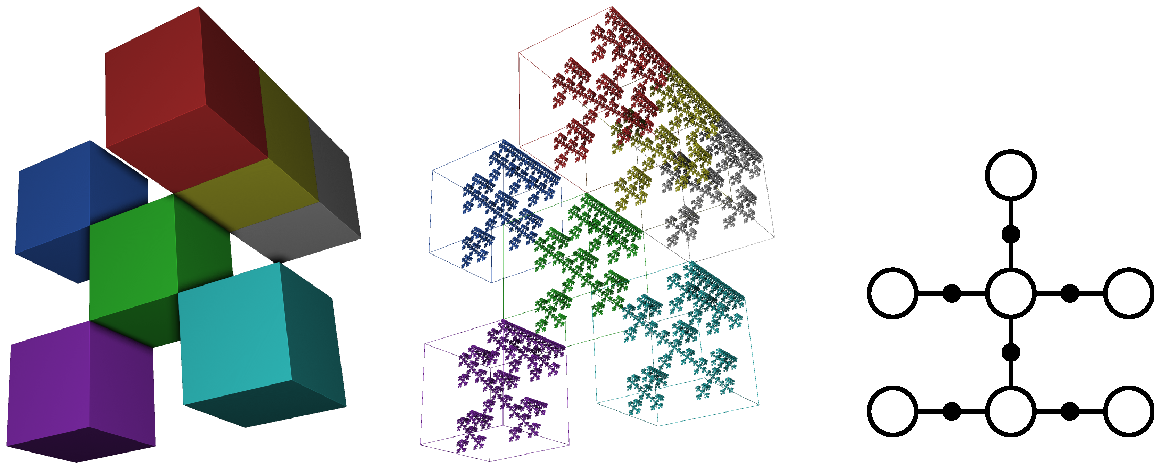
\includegraphics[width=.9\textwidth]{FQ_den.pdf}
    \caption{Фрактальный куб, являющийся дендритом, и его двудольный граф пересечений}
    \label{fig:BMM2022}
\end{figure}

%\begin{example}[Фрактальный куб с одноточечным пересечением]
%Возьмем фрактальный куб $K=\dfrac{K+D}{4}$ с множеством единиц 
%\begin{equation*}
%\begin{split}
%D=\{
%    &(0,0,0), (1,1,1), (2,2,2), (3,3,3), (2,1,1), (1,2,1), (1,1,2),\\ 
%    & (1,2,2),(2,2,1), (2,1,2), (0,0,2), (0,2,1), (3,3,1), (3,1,1),\\ 
%    & (2,0,0), (1,2,0),(1,3,3), (1,1,3)\}     
%\end{split}
%\end{equation*}
% 
%\begin{figure}[H]
%    \centering
%    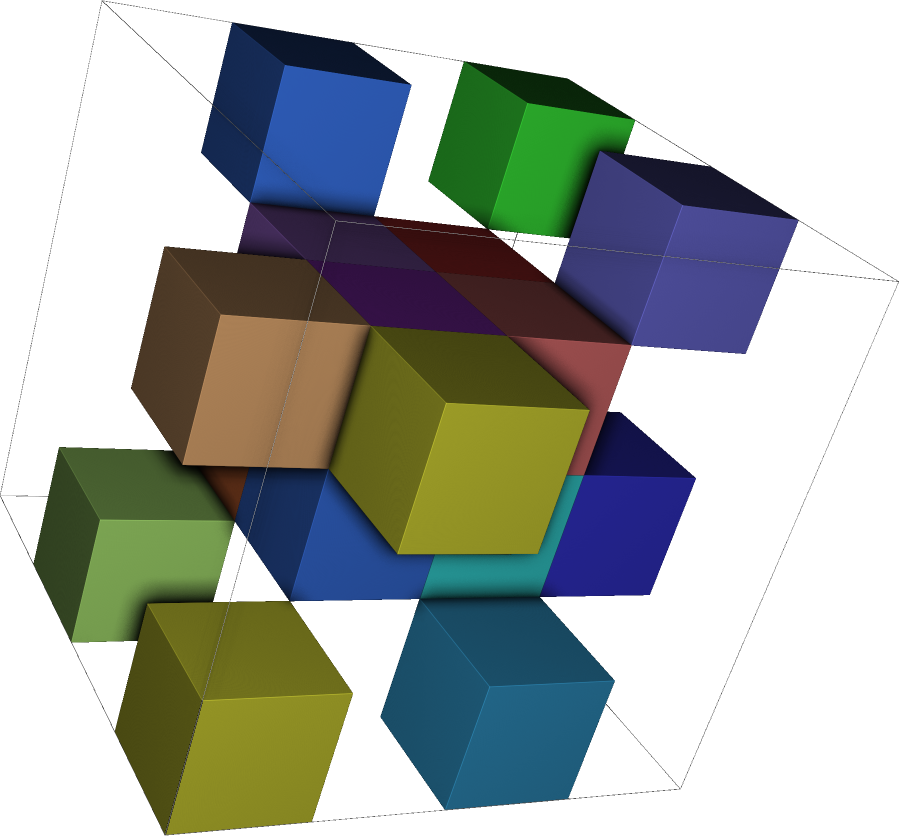
\includegraphics[width=0.45\textwidth]{fqP1a.png}
%    \hfill
%    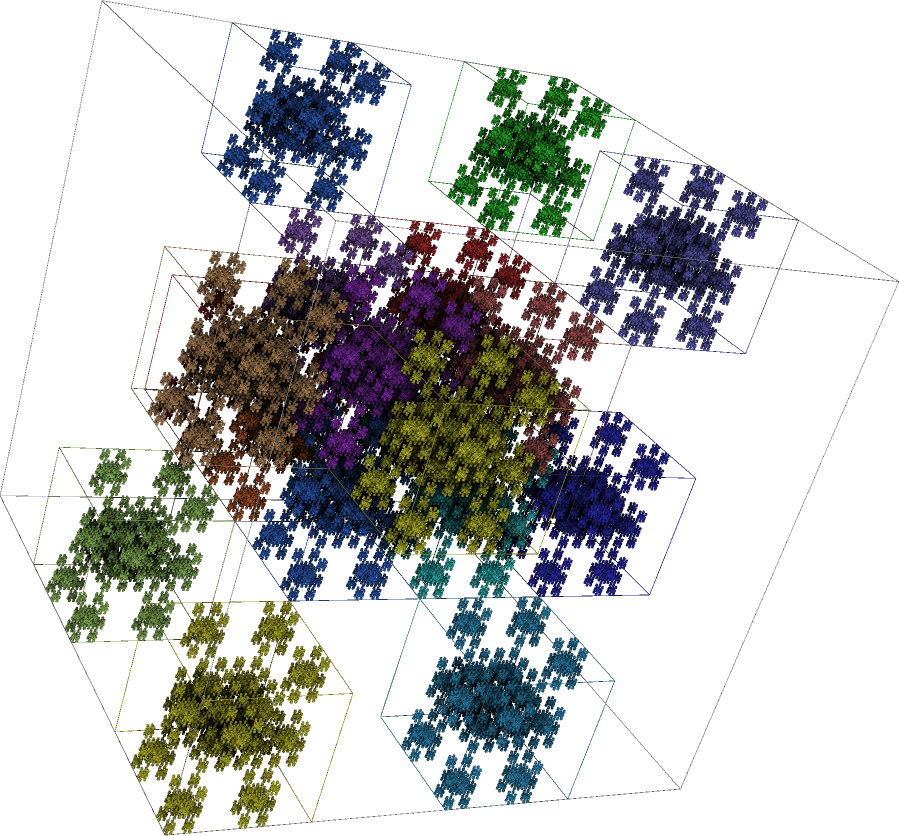
\includegraphics[width=0.45\textwidth]{fqK1a.png}
%    \caption{Фрактальный куб с одноточечным пересечением}
%    \label{fig:fq}
%\end{figure}
%
%\begin{figure}[H]
%    \centering
%    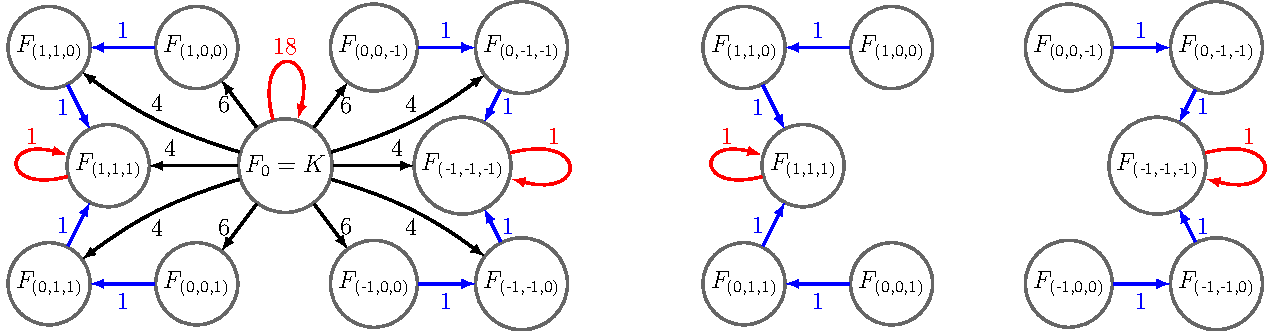
\includegraphics[width=\textwidth]{SG_for_FQ.pdf}
%    \caption{Структурный граф}
%    \label{fig:fq_sg}
%\end{figure}
%\end{example}